87. $f(x)=\cfrac{2-|x+3|}{x}=\begin{cases} \cfrac{2+x+3}{x},\ x\leqslant -3,\\ \cfrac{2-x-3}{x},\ x > -3.\end{cases}=\begin{cases} 1+\cfrac{5}{x},\ x\leqslant -3,\\ -\cfrac{1}{x}-1,\ x > -3.\end{cases}$
$$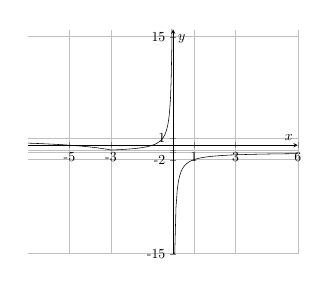
\begin{tikzpicture}[scale=0.5]
\begin{axis}[
    axis lines = middle,
    grid=major,
    legend pos={south west},
    xlabel = {$x$},
    %xlabel style={below right},
    ylabel = {$y$},
    ymin=-15,
    ymax=16,
    xmin=-7,
    xmax=6,
    xtick={-5, -3,1,3,6},
    xticklabels={-5,-3,1,3,6},
    ytick={-15,-2,-1, -0.666,1, 15},
    yticklabels={-15, -2,$ $,$ $,1, 15},
                  ]
    \addplot[domain=-10:-3, samples=100, color=black] {1+(5/x)};
	\addplot[domain=-3:-0.01, samples=100, color=black] {-1-(1/x)};
    \addplot[domain=0.01:6, samples=100, color=black] {-1-(1/x)};
    %\addplot[domain=2.01:6, samples=100, color=black] {2/(2-x)};
   % \addplot[domain=-3:3, samples=100, color=black] {-x};
     %\addlegendentry{$\text{Рис. 1}$};
\end{axis}
\end{tikzpicture}$$
По графику определим ответ $x\in(-\infty;-0)\cup[1;+\infty).$\\
